\documentclass[10pt,a4paper]{article}
%\usepackage[latin1]{inputenc}
\usepackage{amsmath}
\usepackage{amsfonts}
\usepackage{amssymb}
\usepackage{graphicx}
\DeclareMathOperator*{\argmax}{\arg\!\max}
\author{Pavel Gladyshev$^\dagger$, Joshua I. James$^\ddagger$\\
	pavel.gladyshev@ucd.ie, joshua@cybercrimetech.com\\
	$^\dagger$ Digital Forensic Investigation Research Group: Europe\\
	University College Dublin, Belfield, Dublin 4, IE\\
	$^\ddagger$ DFIRE Labs, Legal Informatics and Forenisc Science Institute\\
	Hallym University, Chuncheon, South Korea}
\title{Decision Theoretic File Carving Based on Cluster Sampling}
\date{}
\begin{document}
\maketitle

\begin{abstract}
\noindent Abstract
\noindent\textbf{Keywords:} Decision-theoretic file carving; File carving; Digital Forensic Investigation; Digital Forensic Triage; Preliminary Analysis
\end{abstract}

\section{Introduction}

Digital forensic investigations must process large amounts of evidential data with limited resources \cite{Casey2009, pollitt2013triage}. Modern solutions to the data processing problem combine advances in automatic detection of relevant data with some form of selective human exploration to identify sample data and to validate output results \cite{marturana2013machine, schell2007cyber, james2014measuring}. Despite significant time and cost savings that automation can bring to digital investigations, this approach still relies on exhaustive processing of the suspect data.

Various methods have been proposed that attempt to prioritise exhibits by first prioritising suspect data sources that the exhibit contains \cite{shaw2013practical, rogers2003role, overill2013triage}. Several works \cite{Koopmans2013,Casey2009} have discussed the idea of digital forensic triage; an investigation processes with the goal of not always requiring an exhaustive search of all devices, and helps with decisions of relevancy and prioritisation.

There are many situations where a digital investigator is limited either in time or available computational power. For example, a parole officer may use a portable forensic tool to periodically check that an offender's computer does not contain child abuse material. The time and processing power available to the officer on site is limited and -- given the growth in data storage capacity -- may not be sufficient to exhaustively explore the contents of an offender's computer. Thus a solution is required that would combine automatic processing with probabilistic sampling and prioritisation aimed at discovering relevant information more quickly.

This paper explores the idea of automatic prioritisation and sampling from theoretical and practical standpoints, and demonstrates its viability by example of JPEG image carving.

\subsection{Contribution}
This work contributes to the field of digital forensic investigation by proposing a limited-resource, file carving method that is suitable for digital forensic triage purposes as defined by \cite{Koopmans2013}. Specifically, this work provides:
\begin{itemize}
	\item{a rigorous statement of the problem of digital forensic investigation with limited resources by viewing digital forensics as a decision problem}
	\item{a decision-theoretic approach to file carving that is able to recover up to half of all JPEG files on a disk with 10\% of the processing time}
	\item{demonstrated viability of the proposed approach by constructing a JPEG image carving application that finds potentially relevant images (photographs) faster than traditional carvers}
\end{itemize}

\section{File Carving Approaches}
File carving is often used in digital investigations, and a number of file carving techniques have been proposed. Traditional file carvers, such as foremost \cite{richard2005scalpel} or photorec \cite{grenier2007photorec}, examines the disk blocks in a linear fashion -- starting at the beginning of the drive and working its way towards the end of the drive. Figures \ref{fig:linear_vs_deca}a and \ref{fig:linear_vs_deca}b show typical plots of $WC(t)$ and $pc(t)$ for such a linear file carver. 

\begin{figure}
	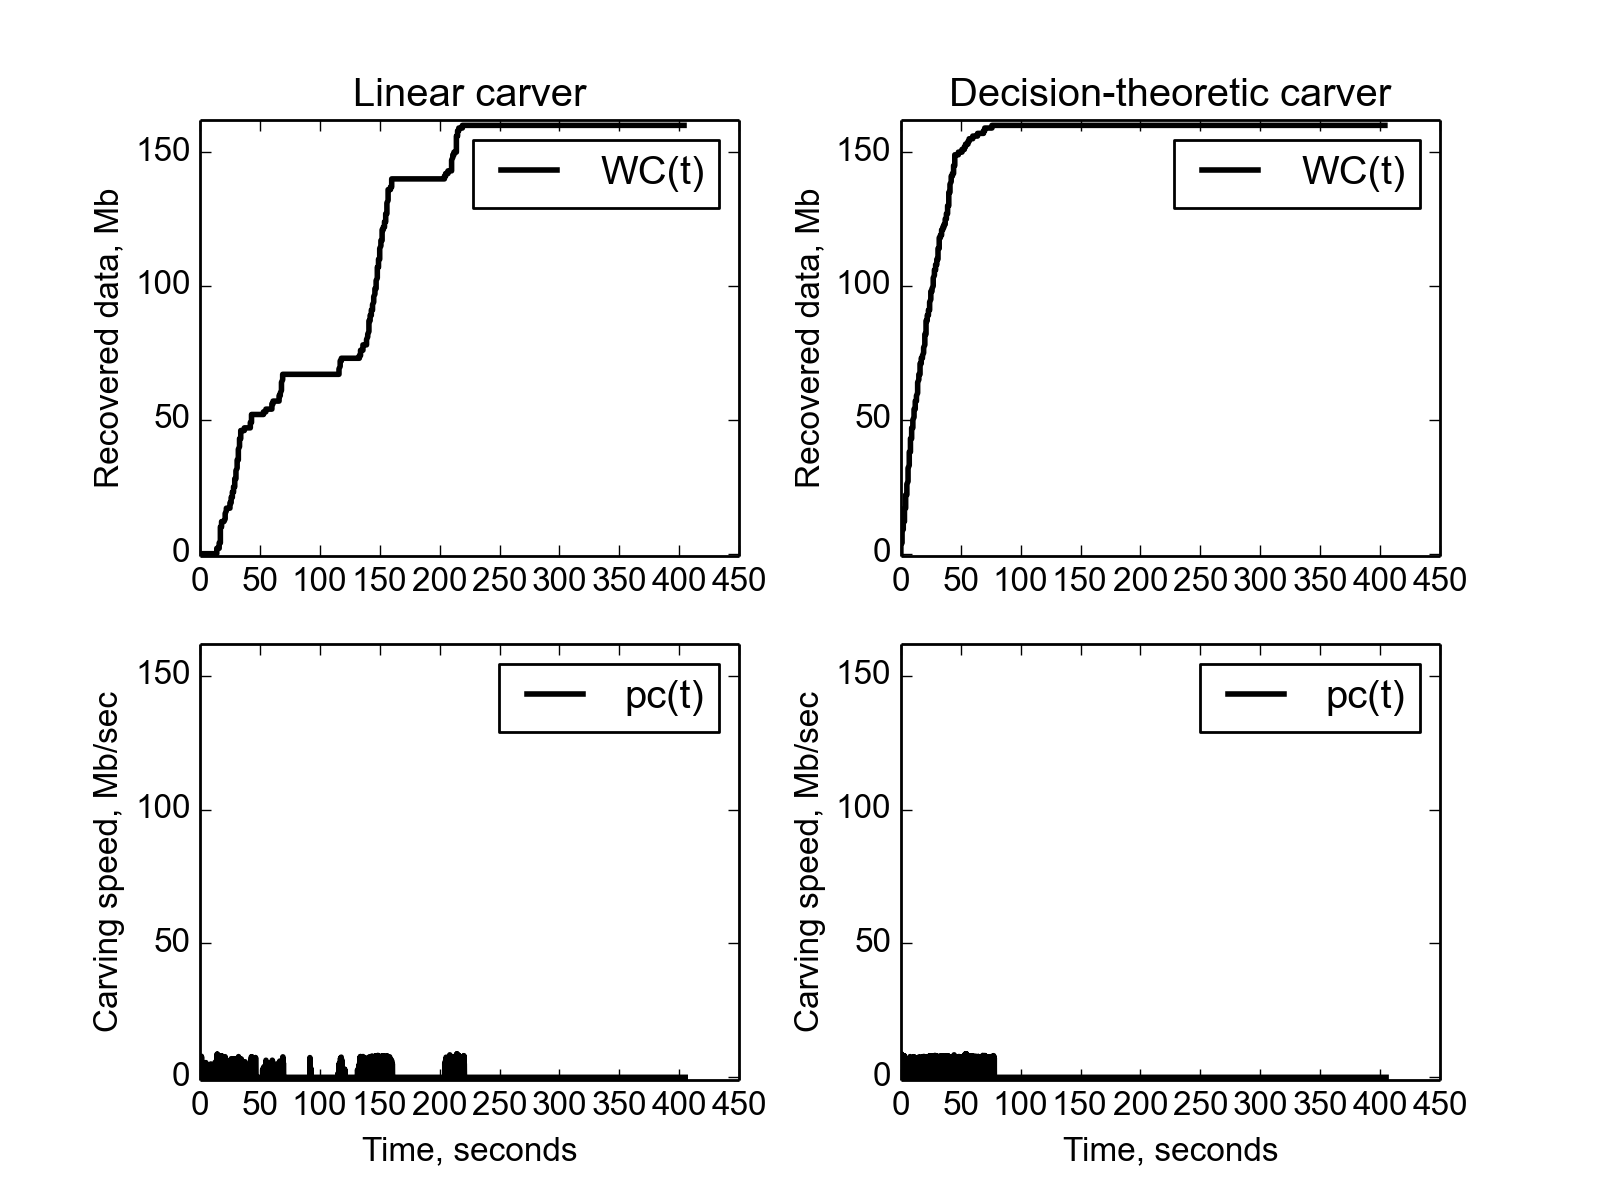
\includegraphics[width=\textwidth]{fig1}
	\caption{Performance of linear vs decision-theoretic carver.}
	\label{fig:linear_vs_deca}
\end{figure}

 If the relevant data is spread uniformly over the disk space, the traditional carvers could take long time to find most of it.

Richard, et al \cite{Richard2007inplace}, and similarly Meijer \cite{MeijerRob2012}, proposed in-place\footnote{Also known as zero-storage} file carving in an attempt to lower the time and space requirements compared to traditional linear carving. These approaches identify the challenges with traditional file carving, and propose methods to reduce carving resource requirements by minimizing the amount of disk I/O associated with copying all file data. Essentially, once file data is discovered, pointers are created in virtual file systems that point to the data directly on the suspect disk rather than copying data from the suspect disk. However, the approach used to determine if a block contains file data is still linear, as before.

Hash-based: \cite{Garfinkel2015hashbased}
Fragment  / Cluster classification: \cite{Veenman2007statistical} \cite{li2011novel}
%
% Check
% https://www.semanticscholar.org/paper/47c06511c3419f628edeabe65e2337fb6844747b
% https://www.semanticscholar.org/paper/74ff9f089da65519466cb770e9a63486ce3a6baa
% Bulk_extractor http://www.sciencedirect.com/science/article/pii/S0167404812001472

%% It should be stressed somewhere that theheader/footer carving approach works because 
%% all of the existing mainstream file systems try to allocate blocks sequentially
%% because sequential access on HHDs is the fastest. 
%%
%% I checked and YAFFS also tries to write file sequentially, because it erases 
%% flash memory in blocks, so it tries to put one file into into one block to avoid
%% the need to relocate pages to a nother block when only a section of the block needs 
%% to be erased.

\section{Decision-theoretic File Carving}

The main objective of a file carver is to recover as much relevant data as possible, while producing little spurious results. Prior research efforts primarily focused on achieving this objective. Nowadays, the capacity of the data storage encountered in investigations made file carving a time consuming process and it is important to start thinking about making the file carving \emph{quick} as well as precise. To put it into perspective, consider that if a forensic workstation takes 400 seconds to process a 32Gb hard disk drive, it would take it more than 10 hours to process a 3 Tb hard disk drive. 

This paper describes an adaptive file carving algorithm that uses initial probing to estimate where the relevant information is likely to be on the drive, and uses this estimate to guide the file carving process.

To explain this idea more precisely, let's introduce two mathematical functions. Let $WC(t)$ denote the amount of relevant data extracted by the carver at the time $t$ since the start of carving, and let $pc(t)$ denote the \emph{carving speed} -- the rate at which the file carver produces relevant data. For the purposes of this paper we define $pc(t)$ to be a difference
\begin{equation}
    pc(t) = WC(t+h) - WC(h)
\end{equation}
over some small time interval $h$.

Alternatively, file carvers could use a heuristic model to \emph{guess} which data blocks are most likely to contain relevant data and prioritize examination of those blocks. If the guessing is sufficiently precise and if the analysis of the guessed blocks can be done efficiently\footnote{We foresee a reasonable objection from our reader that on hard disk drives the sequential access to the data is orders of magnitude faster than random access, but we defer this discussion until Section X. It suffices to say that the development of solid state drives and the evolution of RAMCloud \cite{ousterhout2010case} and similar technologies provide valid business cases for the decision-theoretic file carving.}, the carver will recover most of the relevant data at the beginning of the carving process as shown in Figures \ref{fig:linear_vs_deca}c and \ref{fig:linear_vs_deca}d.

A very basic implementation of this idea is described in the following sections. Despite its simplicity, in our experiments it could recover up to half of all JPEG files from the disk image during the initial 10\% of the processing time. 

The ability to deliver a lot of relevant data quickly, could make such file carving usable in time-sensitive situations, such as digital forensic triage or on-scene investigations, where file carving is not normally used due to the long wait required. 

\section{DECA algorithm}

There are many games like Battleships, Minesweeper, and the Colossal Cave Adventure in which player explores an unknown environment. It is instructive to consider file carving as an analogy of the battleships game shown in Figure \ref{fig:battleships_example}. 

\begin{figure}
  \centerline{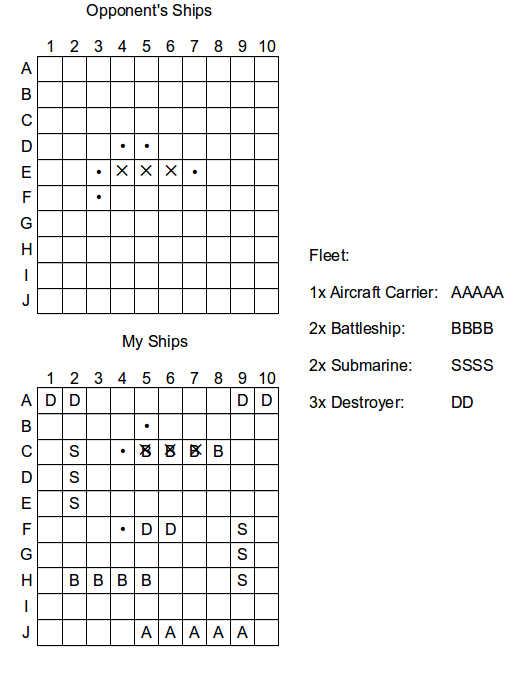
\includegraphics[width=\textwidth]{fig2}}
  \caption{Battleships playing pad.}
  \label{fig:battleships_example}
\end{figure}

According to \cite{Battleships1931} the Battleships game originated in Russia in the pre-World War I days. Each player has a pad of paper with two 100-square grids -- one for arranging the player's ships and the other for noting the discovered locations of the opponent's ships. Every square on a grid is identifiable by a letter and a number. Before the start of the game, each player secretly arranges their ships on their grid. A ship occupies a number of consecutive squares and is oriented either vertically or horizontally. The ships cannot overlap. The game proceeds in turns with each player sending a "bomb" to a particular square on the enemy grid. The other player then responds whether the "bombing" succeeded in damaging one of their ships. A ship is destroyed when all of the squares it occupies has been bombed. The game ends when one of the players completely destroys the other player's fleet. 

A typical strategy is to send random bombs until one of them hits an opponent's ships. The subsequent bombings are used to determine the orientation of the damaged ship and to completely destroy it by targeting the  squares adjacent to the initial hit. What makes this strategy possible is the \emph{a-priori} knowledge of  the placement rules and of the dimensions of the opponent's ships.

Imagine now that instead of a square field the Battleship game is played on a long canal with the opponent's ships situated along it as shown in Figure \ref{fig:battleships_on_a_canal}. A ship occupies a number of consecutive game squares, and -- like before -- ships cannot overlap. A turn consists of the player bombing a particular square along the canal aiming to destroy the enemy fleet with the minimal number of bombs dropped. We hope that the analogy with file carving is self evident. 

\begin{figure}
  \centerline{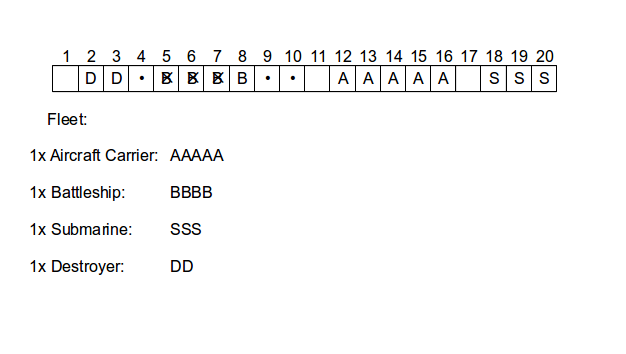
\includegraphics[width=\textwidth]{fig3}}
  \caption{A 1-dimensional Battleships game.}
  \label{fig:battleships_on_a_canal}
\end{figure}

The simplest strategy that is guaranteed to destroy the enemy fleet in Figure \ref{fig:battleships_on_a_canal} is to bomb all squares consecutively from from left to right, which corresponds to the traditional file carving approach. This strategy, however, is not the most efficient if the player has some prior information about the parameters of the fleet and/or its location along the canal. For example, if it is known that all ships occupy hundreds of adjacent squares, then if a bomb hits a ship in some square, then it is very likely that the immediately adjacent squares also belong to the same ship and that another ship is likely to be situated hundreds of squares in either direction of the damaged ship. Like a battle ships game player, DECA algorithm first searches for a file to carve by sampling previously unexplored disk blocks, and then -- once a block belonging to the relevant file is found -- it examines the nearby blocks to find the beginning and the end of that file. We presently ignore file fragmentation and assume that the beginning and the end of the file can be detected using magic signatures. Similar assumptions are made by popular file carvers, such as Scalpel \cite{richard2005scalpel} and Photorec \cite{grenier2007photorec}.

\subsection{Decision theoretic analysis of file carving}

Decision theory offers a well-developed mathematical apparatus for reasoning about decision making. It models decision making as a choice problem where the decision maker has to choose one of several possible mutually exclusive actions to perform: $A=\left\{A_1,A_2,\dots,A_n\right\}$. There is a finite set of mutually exclusive outcomes $O=\left\{o_1,o_2,\dots o_m \right\}$ that may result from performing an action, and each outcome has a certain probability of happening if a particular action is chosen: $P(o_i \mid A_j)$. The desirability of an outcome is modelled by the utility function $u: O \rightarrow \mathbb{R}$ that assigns a numeric value to each outcome. The higher utility values correspond to more desirable outcomes. Decision theory shows that in this setting the right thing to do is to choose an action with the highest mathematical expectation of the utility value across all possible outcomes:

\begin{equation} \label{eq:decision}
\argmax_{i}\sum_{j=0}^m P(o_j \mid A_i )u(o_j)
\end{equation}

The first phase of DECA algorithm is concerned with sampling of unexplored disk blocks. Initially all blocks are unexplored, and the algorithm has to choose which of the $n$ available blocks ($b_0 \dots b_n$) to examine. There are two possible outcomes of each action: the chosen block belongs to a relevant file (i.e. the file of the kind we are trying to carve) or the block contains irrelevant data. This can be modelled by the predicate $rel(b_i)$, such that $rel(b_i) = T$, if the block $b_i$ belongs to the relevant file and $rel(b_i) = F$ otherwise. Clearly $P(rel(b_i) \mid i) + P(\neg rel(b_i) \mid i) = 1$ and $P(rel(b_i) \mid i) = 1-P(\neg rel(b_i) \mid i)$.  Let's initially ignore the cost of examination of non-adjacent disk blocks imposed by the hard disk drive seek time, and assume a very simple utility function:

\begin{equation}
u(i)= \begin{cases}
      1 & rel(b_i) \\
      0 & \neg rel(b_i)
      \end{cases} 
\end{equation}

The formula \ref{eq:decision} then simplifies to $\argmax_{i} P(rel(b_i) \mid i)$, meaning that the algorithm should choose to examine the block with the highest \emph{a-priori} probability of being part of relevant file. 

Observe that there are cases when all unexplored blocks have equal probability of containing relevant data. This could happen, for example, while carving images from unallocated space on an old CCTV system, where all of the unexplored blocks are known to contain fragments of relevant files and the carver just needs to identify start and end of each fragment.  Linear carver is optimal in these circumstances, because it will always find relevant data by examining the next unexplored block. The same is true if we aim to recover /emph{all} the data from the unexplored blocks\footnote{Note that while file carvers are routinely used to recover all possible data, typically only a small fraction of that data is useful as evidence or intelligence. Most file carvers can be configured to limit file extraction to only particular kinds of files.}. 

If the aim is to recover a \emph{specific} type of data, such as digital photographs, digital video, and audio recordings, there is usually prior information that could be used to to speed up the carving process by prioritizing examination of the unexplored blocks. This is demonstrated in the rest of this paper. We use the fact that raw digital photographs tend to be large to compute an estimate of $P(rel(b_i) \mid i)$ and then use this estimate to gain a speed up when carving raw digital photographs.

\subsection{Estimating $P(rel(b_i) \mid i)$ for raw digital photographs}

A digital camera sensor produces raw photographs at a fixed resolution. The raw sensor data is resized by the camera to fit the selected output resolution, and compressed. The resulting file is, typically, several megabytes in size. Recall that JPEG image is divided into a number of $8 \times 8$ pixel fragments before compression, and each fragment is compressed independently. By the central limit theorem, the overall size of JPEG file should obey normal (Gaussian) distribution. Figure \ref{fig:jpeg-dist} shows a histogram of file sizes of a personal collection of raw digital photographs accumulated over a period of 10 years. There are several peaks corresponding to different cameras and image quality settings used over the years. Note, however, that each peak follows the normal distribution.

\begin{figure}
  \centerline{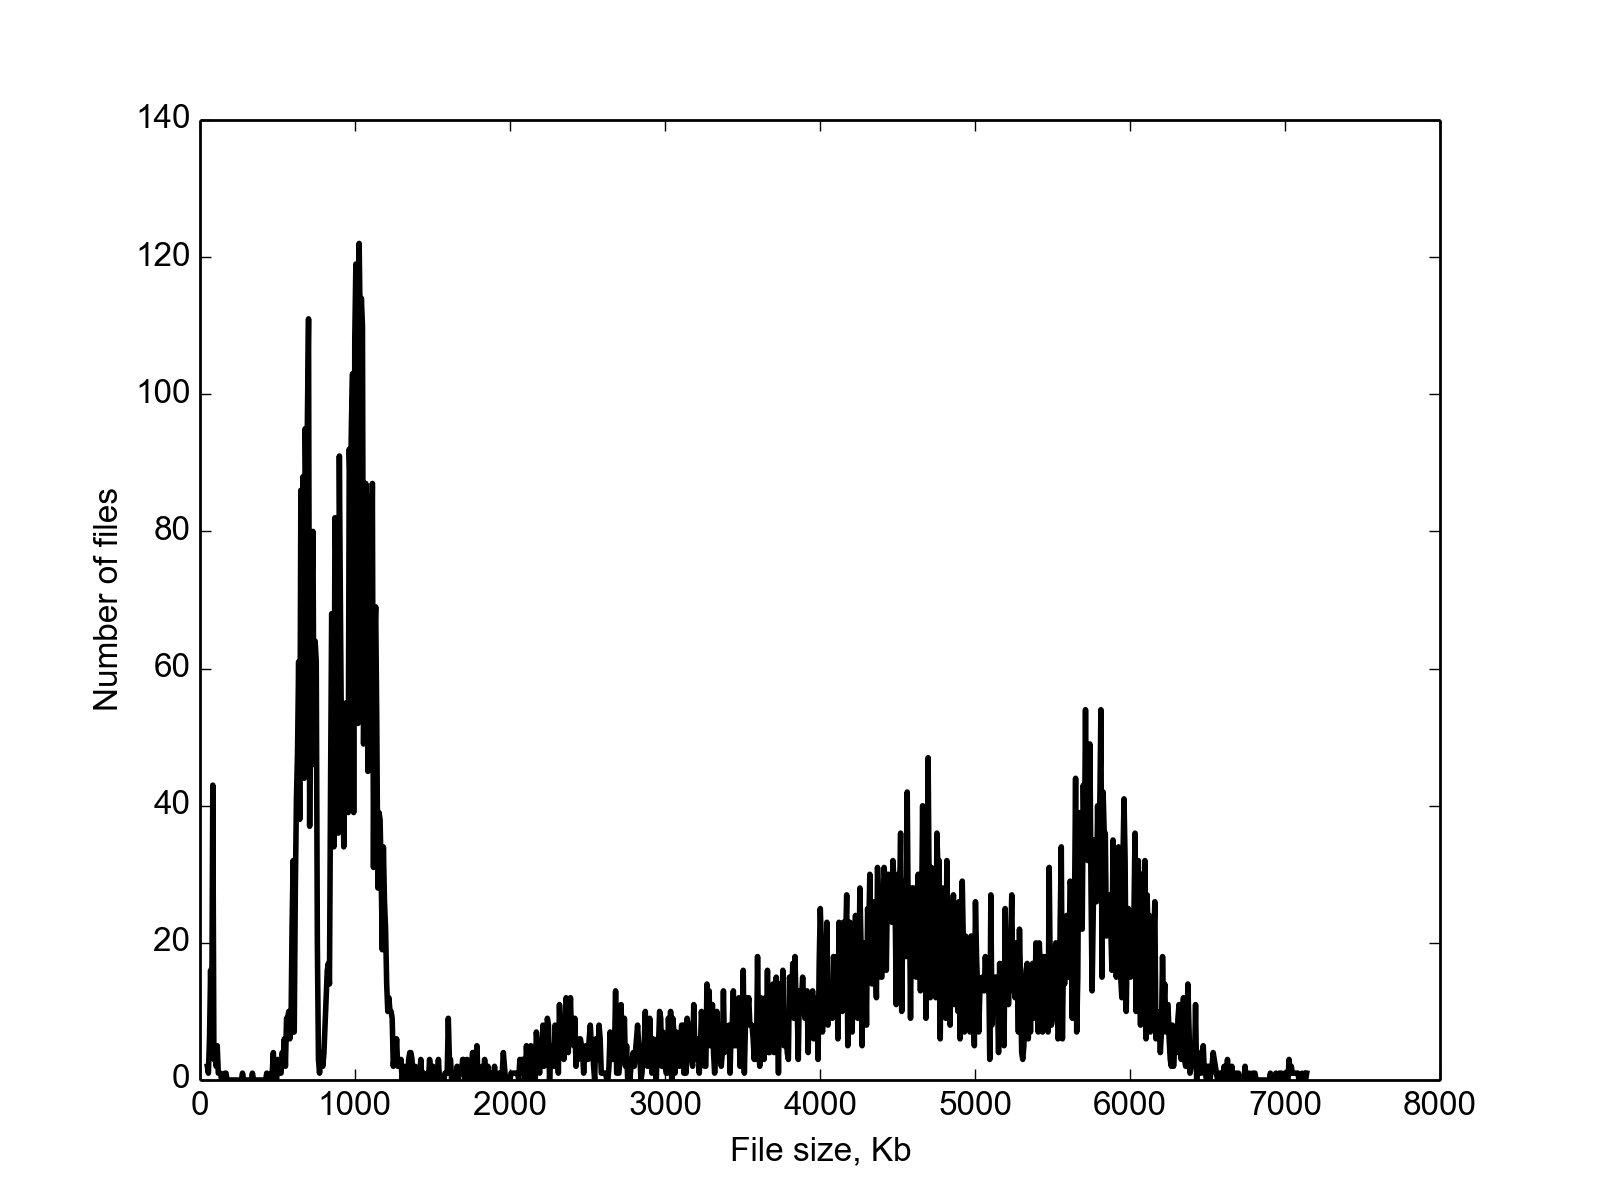
\includegraphics[width=\textwidth]{jpeg-sizes}}
  \caption{Histogram of file sizes (in 1 kilobyte blocks) of a personal collection of raw digital photographs in JPEG format. Each of the peaks visible in the histogram correspond to different cameras and image quality settings used over the years.}
  \label{fig:jpeg-dist}
\end{figure}


To get a sense for probability distribution $P(rel(b_i) \mid i)$ a series of stochastic simulations had been performed. Each simulation generated approximately 20 simulated image files. The simulated files were ''stored'' at random\footnote{The uniform distribution was assumed.} locations throughout the disk block array. $P(rel(b_i) \mid i)$ was then estimated as the frequency of a particular $b_i$ being ''allocated'' to an image file. The files were always stored in consecutive blocks of disk space (i.e. there was no file fragmentation).

\begin{figure}
  \centerline{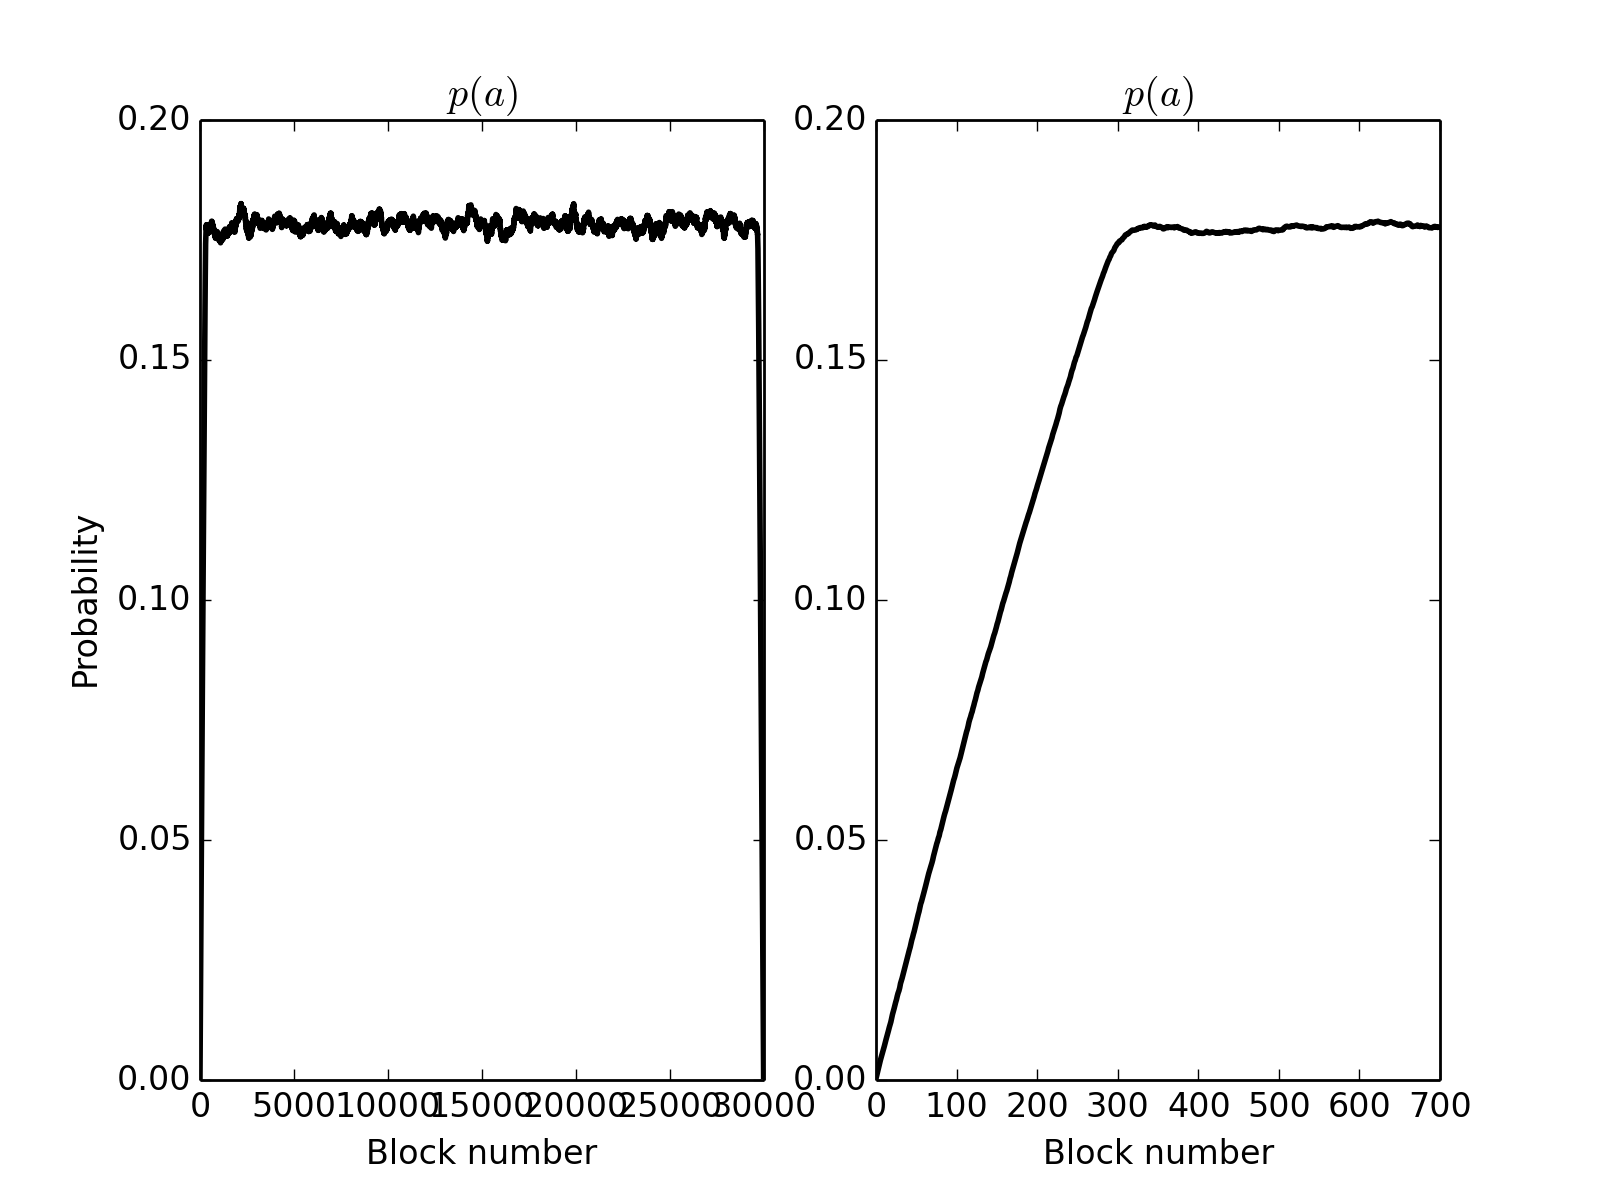
\includegraphics[width=0.9\textwidth]{fig4}}
  \caption{An estimate of $P(rel(b_i) \mid i)$ computed by stochastic simulation. The average size of generated files is 300 blocks, the disk block array consists of 30,000 blocks. The left plot shows the entire distribution. The right plot is a zoom-in of  $P(rel(b_i) \mid i)$ to the initial segment of 700 blocks.}
  \label{fig:montecarlo}
\end{figure}

Figure \ref{fig:montecarlo} shows the estimate of $P(rel(b_i) \mid i)$ after $10^6$ simulations. The average size of the simulated files was kept at 300 blocks and the disk block array contained only 30,000 blocks. Observe that the probability of finding an image file by testing $b_0$ is much lower than the probability of finding an image file by testing a block at some distance from the beginning of the disk. The probability $P(rel(b_i) \mid i)$ reaches maximum around the block $b_{300}$, where 300 is the average file size of the generated files. The reason for that is the assumed absence of fragmentation, normal (Gaussian) distribution of simulated file sizes, and random (uniform) distribution of starting positions of the files in the drive array\footnote{Consider the following informal argument: the block $b_0$ can only be the first block of a continuous 300-block file, while the block $b_{300}$ could be part of a continuous 300-block that starts in \emph{any} of the positions $i=0 \dots 300$. Thus, $b_{300}$ is 300 times more likely to be part of the relevant file than $b_0$, if all possible starting positions of the file are \emph{equally} likely.}.  


\begin{figure}
  \centerline{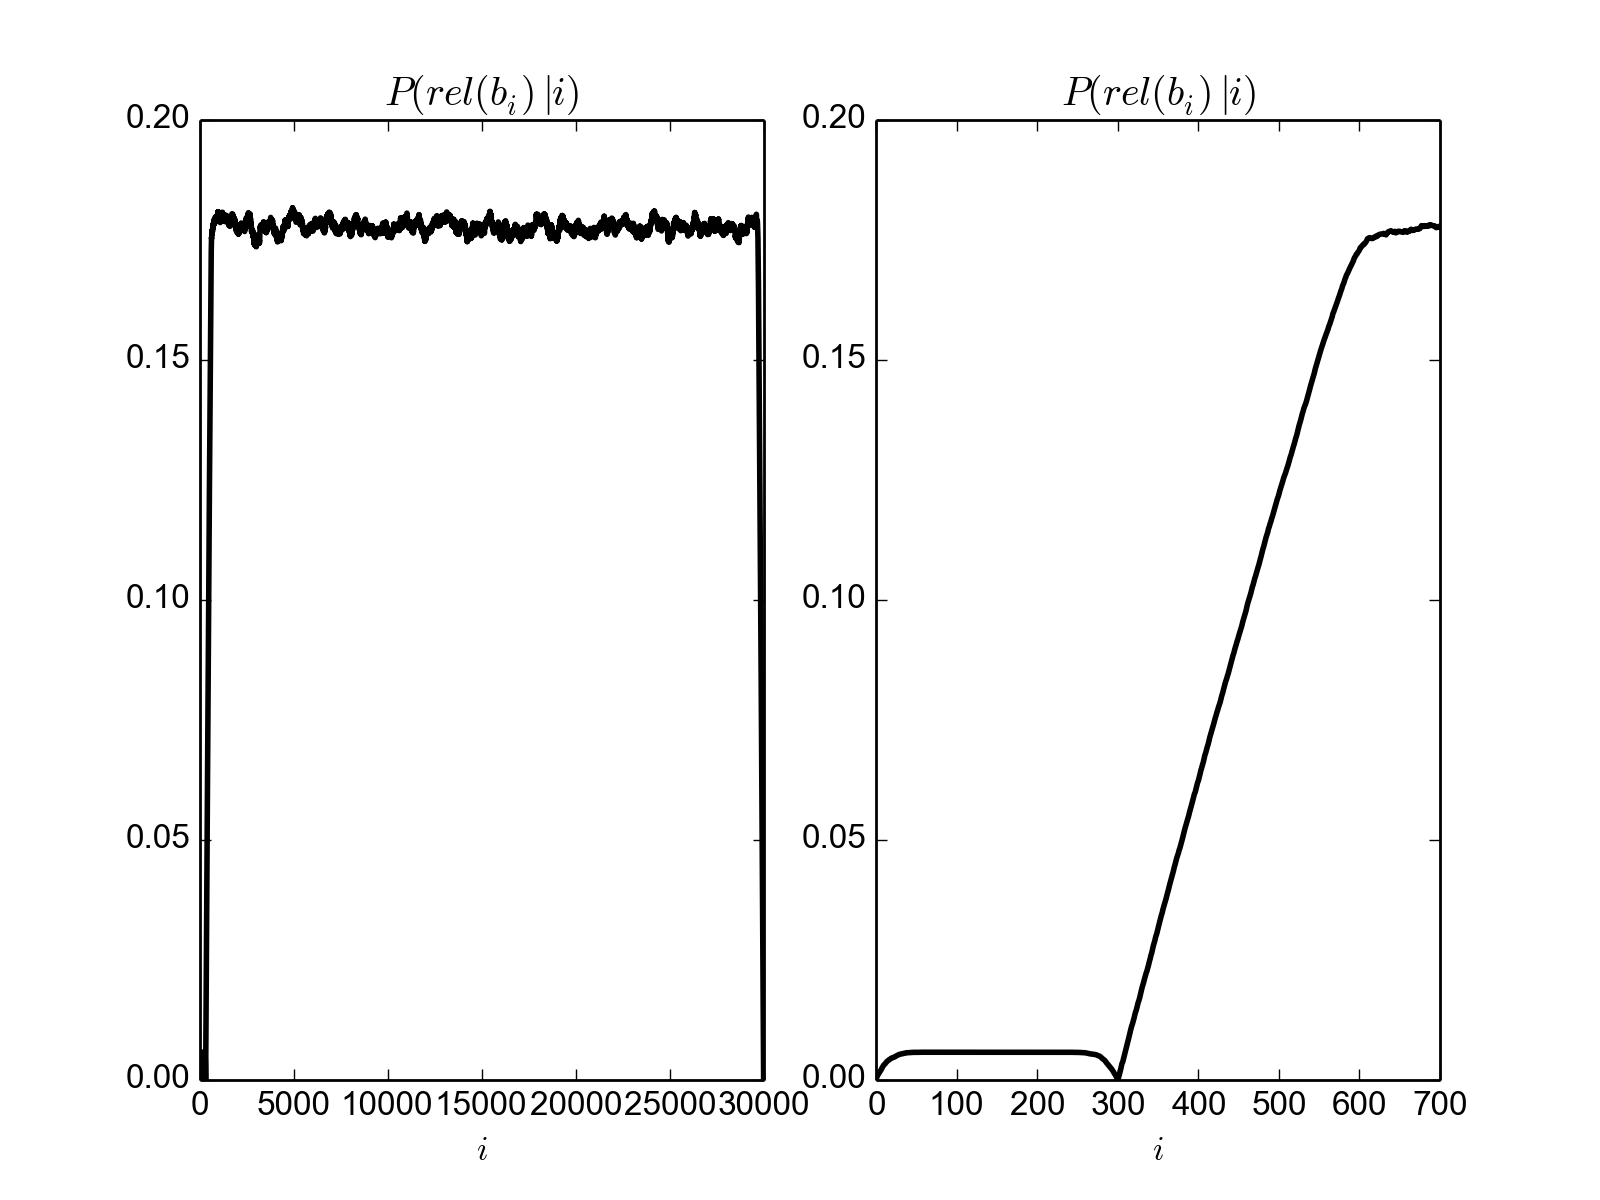
\includegraphics[width=0.9\textwidth]{fig4_1}}
  \caption{An estimate of $P(rel(b_i) \mid i)$ counting only simulations where block $b_{300}$ was tested and found to contain \emph{irrelevant} data.}
  \label{fig:montecarlo-miss}
\end{figure}

Figure \ref{fig:montecarlo-miss} shows the estimate of $P(rel(b_i) \mid i)$ using a slightly different experiment: we tested the content of $b_{300}$ after each simulation and counted \emph{only} simulations where $b_{300}$ contains irrelevant data. Thus, Figure \ref{fig:montecarlo-miss} models the effect of finding irrelevant data in a certain block on the probability distribution $P(rel(b_i) \mid i)$. Note that the shape of $P(rel(b_i) \mid i)$ to the right of the tested block is virtually identical to the shape of $P(rel(b_i) \mid i)$ in Figure \ref{fig:montecarlo} reaching maximal probability at $i=300+300=600$. The shape of $P(rel(b_i) \mid i)$ to the left of the tested block is also similar to the overall shape of  $P(rel(b_i) \mid i)$ in Figure \ref{fig:montecarlo}, but the maximal probability is much lower because the segment of blocks between $b_0$ and $b_{300}$ is quite small and, consecutively, the chance of a relevant file being there is low. Obviously, no file longer than 300 blocks could fit in $b_0 \dots b_{300}$.

Figure \ref{fig:montecarlo-miss} suggests that testing a block and finding irrelevant data in it can be viewed as splitting the disk block array into two parts with the \emph{posteriori} distribution $P(rel(b_i) \mid i)$ of each part similar in shape to the \emph{a-priori} distribution $P(rel(b_i) \mid i)$ of the initial array. 

If a limit can be put on the \emph{minimal} size of relevant files, Figure \ref{fig:montecarlo-miss} suggests that the relevant files could be detected more efficiently by skipping over multiple blocks while testing for relevant data instead of testing all blocks consecutively. The next secion shows that this is indeed the case, if the non-consecutive examination of blocks does not incur a significant time penalty.

\subsection{Taking into account drive seek time}



Explanation how to incorporate seek time penalty in our model by redefining utility function on the basis of carving time $WC(t)$...


Given that solid state drives are becoming more commonplace in forensic workstations, and taking into account that the majority of files in file system are not fragmented according to \cite{garfinkel2007carving}, we decided to build and evaluate a prototype carver that skips over unexplored blocks instead of examining them sequentially. It is described in Section \ref{sec:implement}.

\section{Implementation and Evaluation of DECA carver} \label{sec:implement}
The previously described DECA algorithm was implemented using C++. The source code can be found at !!!!!!!! CHECK !!!!!!!!!!!!! https://bitbucket.org/pavel\_gladyshev/deca. The software implementation defaults to linear carving mode. Two of the main functions of the software. First, a disk can be sampled to determine its seek time. With seek-time information, an investigator can determine jump distance at which DECA carving becomes faster than traditional linear carving. Second, the software allows for carving using the DECA algorithm while setting the minimal sector jump distance (in 512 sector increments).

Experimentation seeks to demonstrate the theorized performance of the DECA algorithm, and compare the algorithm to other file carvers commonly used in digital investigations.

\subsection{Experimentation Design}
DECA is based on estimates of the distribution of JPEG data on a disk. Based on this estimation, DECA attempts to search only the most likely locations for related data. The result of the DECA algorithm is that some sectors will be skipped. In some cases, skipping sectors that are unlikely to contain relevant data may result in carving speed up. However, this method is also likely to miss smaller files.

DECA, in practical terms, can be described simply. If the jump size is high, carve times and number of carved files will decrease. If the jump size is low, carve times will increase and the number of carved files will increase. As discussed, this depends on the seek time of the disk holding the data to be analyzed. From the prior description, we propose that DECA is most beneficial when attempting to carve a small number of large files from a disk with a low seek time.

From the description of DECA we propose the following hypotheses for testing:
\begin{enumerate}
	\item DECA will have a more significant reduction in run-time as the seek time of the disk decreases compared to other carving methods.
	\item DECA will have a more significant reduction in run-time compared to other carving methods based on the size of disk/image being analyzed.
	\item DECA will normally find a small number of files compared to linear carvers.
	\item DECA is best suited for carving a small number of large files on a low-seek-time disk.
\end{enumerate}

Two disk images were created for testing. One is based on a 4GB USB thumb drive, with a collection of JPEG images along with other documents stored in a FAT32 partition. The second is a 32GB image of a Windows XP operating system containing a user-created documents and JPEG images taken with various digital cameras.

Along with DECA, other carvers tested with the same data sets include Photorec, Scalpel 1.60, Scalpel 2.1 and Foremost. Each of these carvers were configured to only search for JPEG images.

\subsection{Evaluation}
Created disks with data from GovDocs1 \cite{Garfinkel2009}
To test hypothesis 1, each carver was used on the test data set while stored on an sold state drive (SSD) and hard disk drive (HDD). The 4GB image was also tested inside a RAMDisk. RAM cache was cleared before each run. Measurement of carving performance is based on sampling the number of carved files in the carver's output directory (contained on the same disk as the test image) every 0.25 seconds until the carver terminates. All raw test data and testing scripts can be found in the project repository given above.

To determine whether DECA had a more significant reduction in run-time compared to linear carving, we compared the average speed increase over all linear carvers (including DECA in linear carving mode) to the average speed increase between DECA with 7 minimum-file-size configurations (default, 64, 200, 300, 600, 1200, 2400).

The average speed increase for linear carving from HDD to SSD was 237\%. The average speed increase for DECA carving from HDD to SSD was 553\%. The average speed increase for linear carving from SSD to RAMDisk was 327\%. The average speed increase for DECA carving from SSD to RAMDisk was 1229\%. Overall, the average speed increase for linear carving was 298\%, while the average speed increase for DECA carving was 891\%. As expected, when DECA had lower minimum file-size values (64 to 300), performance was equal to or below linear carving on disks with high seek times. Hypothesis 1 is found to be true in most cases except when DECA minimum-file-size is less than 600 on high seek-time disks. The disk seek-time will affect the level of minimum-file-size that should be used.

%\begin{figure}
%	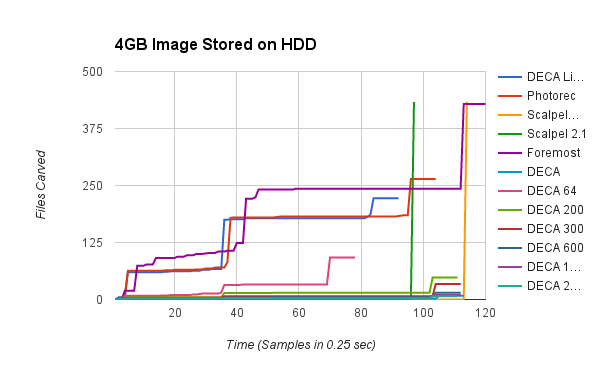
\includegraphics[width=\textwidth]{figures/HDDsmall.png}
%	\caption{DECA carving compared to popular linear carvers where the x-axis is the number of images carved; the y-axis is the number of samples in 0.25 increments; the length of the line is the total time of the carving process on a hard disk drive with a high seek-time. Here DECA carving has similar run times while the minimum-file-size is \textless 600.}
%	\label{fig:HDDsmallAnalysis}
%\end{figure}
%
%\begin{figure}
%	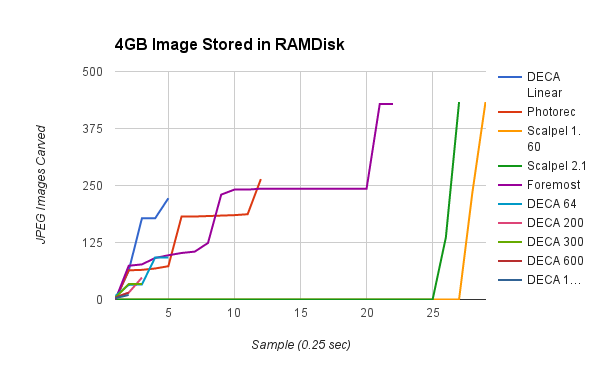
\includegraphics[width=\textwidth]{figures/RAMDISKsmall.png}
%	\caption{DECA carving compared to popular linear carvers where the x-axis is the number of images carved; the y-axis is the number of samples in 0.25 increments; the length of the line is the total time of the carving process on a RAMDisk drive with a low seek-time.}
%	\label{fig:RAMDISKsmallAnalysis}
%\end{figure}

To test hypothesis 2 we calculated the average speed increase for linear carving and DECA carving from HDD to SSD. For the 4GB image, DECA performed 316\% over the linear carver average. For the 32GB image DECA performed 434\% over the linear carver average. Similar to before, if DECAs minimum-file-size was below 600, DECA performed at or below the linear carver average for the 32GB drive. As can be seen in Figure \ref{fig:4v32}, DECA saw greater performance increases from HDD to SSD with a larger disk image when minimum-file-size is greater than 600. This is explained by the cumulative effect of continually skipping large sections of the disk. 

\begin{figure}
	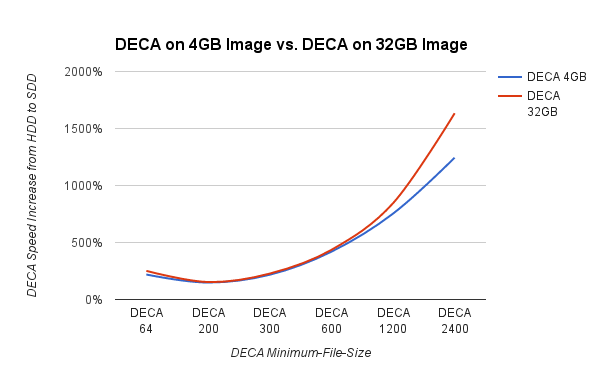
\includegraphics[width=\textwidth]{figures/4GBv32GB.png}
	\caption{DECA time performance improvements in percentage when comparing carving times on an HDD to carving times on an SSD. This graph shows that DECA performs better with larger disk images when minimum-file-size is greater than 600.}
	\label{fig:4v32}
\end{figure}

To test hypothesis 3 we counted the average number of files returned from each carving process. On the 4GB disk image, linear carving returned 356 files on average, and DECA carving returned 30 files on average (regardless of underlying disk). This is consistent with what was predicted since DECA is likely to skip small files and fragments that linear carving will find.

To test hypothesis 4, we examine results of the largest tested DECA minimum-file-size. In our experiments, the largest minimum-file-size used was 2400, which tells DECA that a file is likely to be located within 1,200Kb of its current location. With this setting, DECA was 5 times faster than the linear carving average on an SSD, and 19 times faster than the linear carving average on a RAMDisk. However, DECA only recovered 2\% of the files recovered by linear carving. Overall, it appears that hypothesis 3 is also true. By expanding the minimum-file-size DECA accepts and using a disk with a lower seek-time, DECAs speed will dramatically increase at the expensive of smaller file recovery.

\subsubsection{Discussion}
The DECA algorithm worked as theorized, however, a practical implementation is likely more interesting to investigators. DECA produces significant carving speed increases under certain circumstances, but always at the cost to the number of files carved. Specifically, DECA is ideal for carving a small number of large files across a large, low-seek-time disk. For this reason, DECA may be appropriate for triage purposes, where very fast but incomplete image recovery is acceptable. In cases where the maximum number of files should be carved, or when carving high-seek-time devices (HDD), linear carving largely outperforms DECA.

As discussed, DECA jumps to sections of the disk based on a calculated data distribution. DECA then checks for an image header or footer. If not found, then DECA attempts to classify the data as a JPEG or not. The classifier that was developed could likely be improved. This would increase the number of images correctly recovered, potentially at the cost of speed.

The current implementation of DECA focuses on JPEG images, while imagining current digital cameras that produce images greater than 1 megabyte. However, this algorithm may be suitable for other specific file types, such as music, video, zip files and email containers. This method could also be used in conjunction with other carving methods, such as in-place carving \cite{Richard2007inplace, MeijerRob2012}.

\section{Conclusions}
Decision theoretic analysis allows a file carver to consider the most likely locations of relevant data based on what is currently known about the distribution of data on the disk. By skipping sections of the disk that are unlikely to contain relevant data, carving times can be greatly decreased, where speed benefits are cumulative as the disk becomes larger. Through a practical implementation we demonstrated that decision theoretic analysis is useful when carving a small number of files from a large, low-seek-time disk. With current storage disk technology, decision theoretic carving (DECA) is best implemented as a triage solution. For traditional carving needs, linear carving gives more comprehensive results, and on standard hard disk drives, also has similar carving speeds.

\subsection{Future Work}
This work is a first effort to propose decision theoretic analysis applied to file carving. There are currently a number of limitations to the practical implementation (DECA) carver. Specifically, file distribution has been pre-calculated based on surveyed data in other drives. Future work will attempt to find a method for calculating a data distribution on the disk to be analyzed without increasing carving time significantly. Next, as DECA jumps to a location on the disk it must detect whether the data stored in that location is relevant. We have attempted several detection methods, most of which significantly increased the overall run time. We will seek to improve the data classifier that DECA uses. 

\bibliographystyle{ieeetr}
\bibliography{DECA}
	
\end{document}
